\chapter{Resultados\label{sec:Resultados}}

En el presente capítulo se han recopilado los resultados obtenidos tras cada una de las fases del proyecto. Por motivos de comprensión y presentación, \textbf{aquellos resultados asociados al desarrollo de la \acrshort{PCB} han sido presentados en el capítulo \ref{sec:Implementacion_PCB}} de modo que no se volverán a repetir en este. En caso de que se deseen revisar de nuevo estos se encuentran en el apartado \ref{sec:PCB_Resultados}.

Los siguientes apartados contienen aquellos resultados asociados al desarrollo del software tanto del microcontrolador STM32F4 como del ESP y su comunicación con LabView.

\section{Funcionamiento del ADS\label{Resultados_ADS}}

Para comprobar que el ADS está midiendo correctamente este incluye una señal de \textit{test} conocida cuyas características se encuentran perfectamente definidas en la hoja de características del componente.

Las características de la señal \textit{test} dependen de los bits almacenados en el registro \textbf{Config 2}. Durante la realización de este proyecto se le ha asignado a Config 2 el valor 0xD1 (11010001) para que la señal de \textit{test} se genere de forma interna, con un voltaje que oscila entre $\pm4.5/2400V$ ($\pm1.875mV$) y frecuencia de f$_\text{CLK}$\/$2^{20}$.

La siguiente figura muestra una representación del voltaje real de la señal test comparándolo con la amplitud teórica calculada según la fórmula proporcionada por la hoja de características:

\begin{figure} [H]
    \centering
    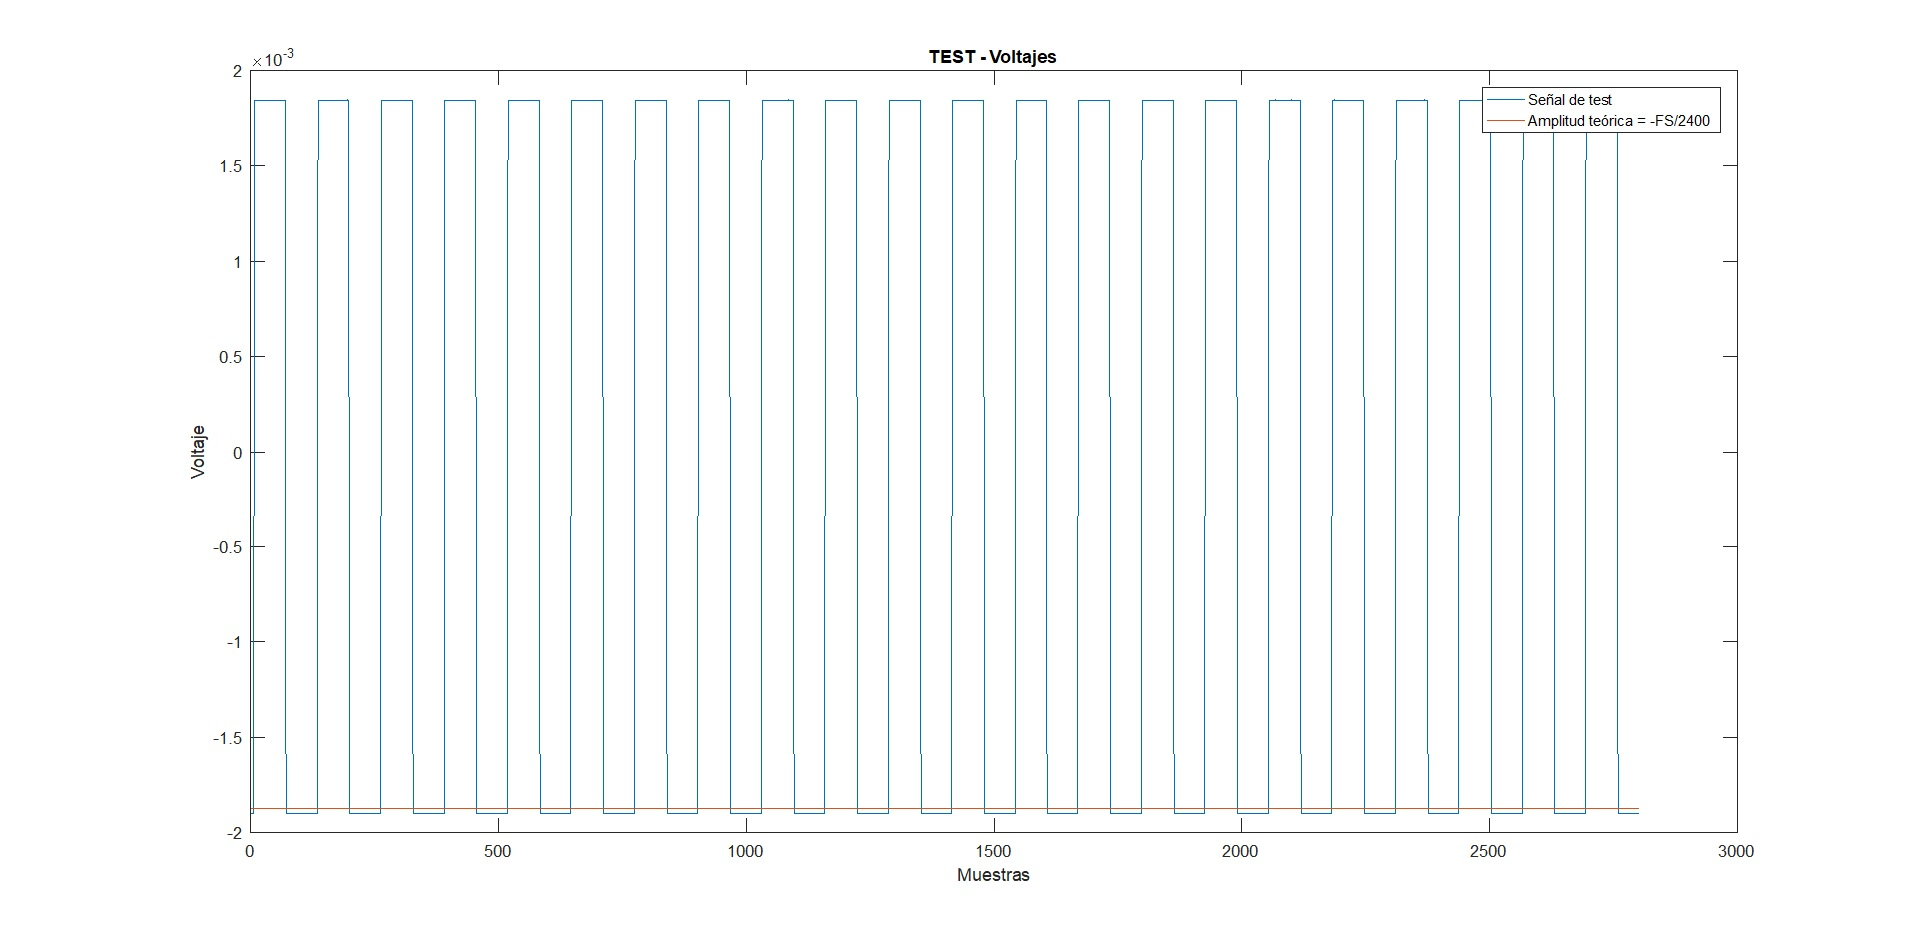
\includegraphics[width=16cm]{Test_teorica}
    \caption{Comparativa entre la señal test y su amplitud teórica}
    \label{fig:tes_teorica}
\end{figure}

Finalmente, tras realizar una medida desde Labview el resultado es el siguiente:

\begin{figure} [H]
    \centering
    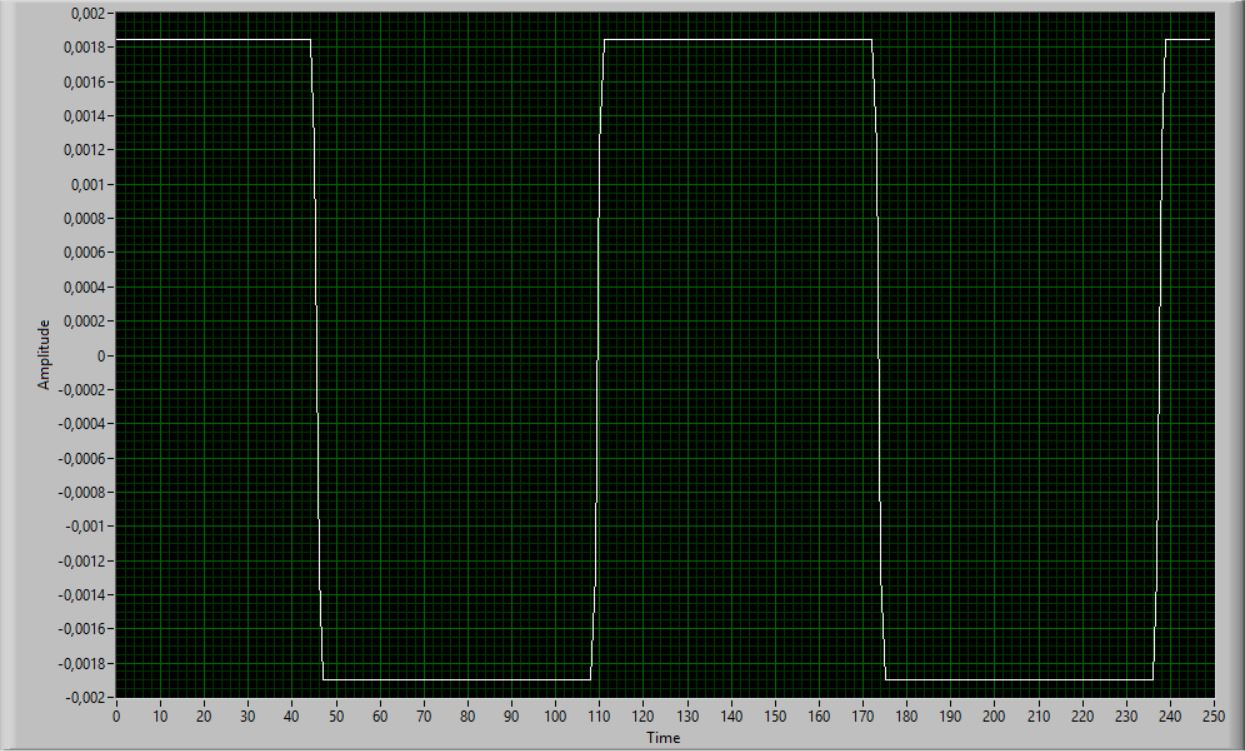
\includegraphics[width=15cm]{Test_limpia}
    \caption{Señal de test medida usando LabView}
    \label{fig:Test_limpia}
\end{figure}

Tras comprobar que se recibe una señal con las características esperadas se puede concluir que el ADS se encuentra correctamente configurado y listo para realizar medidas sobre voltajes reales.

\section{Medidas sobre señales reales\label{Resultados_Medida_Real}}

Las primeras señales reales a medir han sido señales con características conocidas. De esta forma resulta muy sencillo identificar si algún elemento no está funcionando correctamente. Para una prueba inicial se preparó un generador de señales haciendo uso de un Arduino UNO. Esta señal presenta una amplitud que va entre 0V y 5V y una frecuencia de 2Hz. El resultado tras medir esta señal se encuentra representado en la figura \ref{fig:Senal_triangular_saturada}.

\begin{figure} [H]
    \centering
    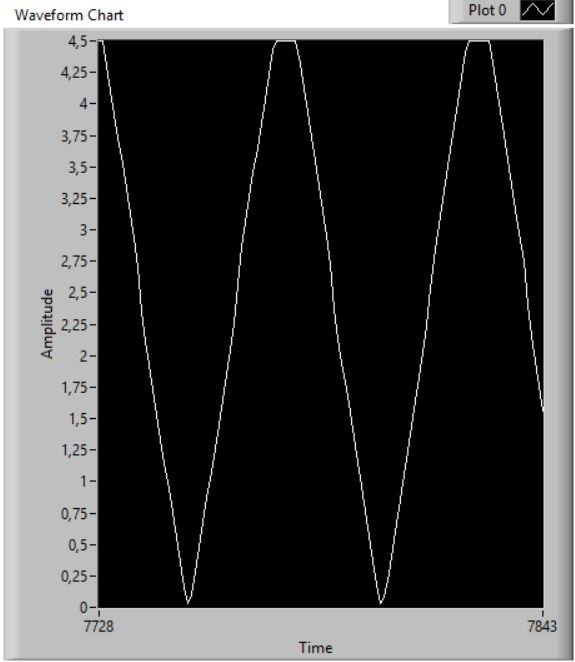
\includegraphics[width=11cm]{Senal_triangular_saturada}
    \caption{Señal real triangular generada con Arduino}
    \label{fig:Senal_triangular_saturada}
\end{figure}

Todos los parámetros se encuentran dentro de los rangos esperados, pero se aprecia una deformación en la señal en los picos superiores del triángulo. Este efecto es debido a la saturación del sistema, pues la amplitud máxima que es capaz de adquirir tanto en positivo como en negativo depende directamente de V$_{\text{REF}}$ (4.5V).

\clearpage

\section{Filtrado de la señal\label{Resultados_filtrado}}

El siguiente paso es aplicar a esas señales reales un filtrado para comprobar que los filtros implementados cumplen con su función.

Siguiendo el ejemplo sugerido por la referencia de CMSIS-DSP se implementó un filtrado de rechazo de banda con el que eliminar las componentes en frecuencia no deseadas de una señal. La señal original es una señal artificial formada por dos senos de distintas frecuencias (10Hz y 50Hz) y el objetivo es eliminar la componente de 50Hz o minimizar su impacto. 

En primer lugar se realizó una estimación del efecto que tendría aplicar un filtro sobre una señal de esas características. El resultadode la simulación realizada en MatLab es el mostrado en la figura \ref{fig:Notch_Matlab}

\begin{figure} [h]
    \centering
    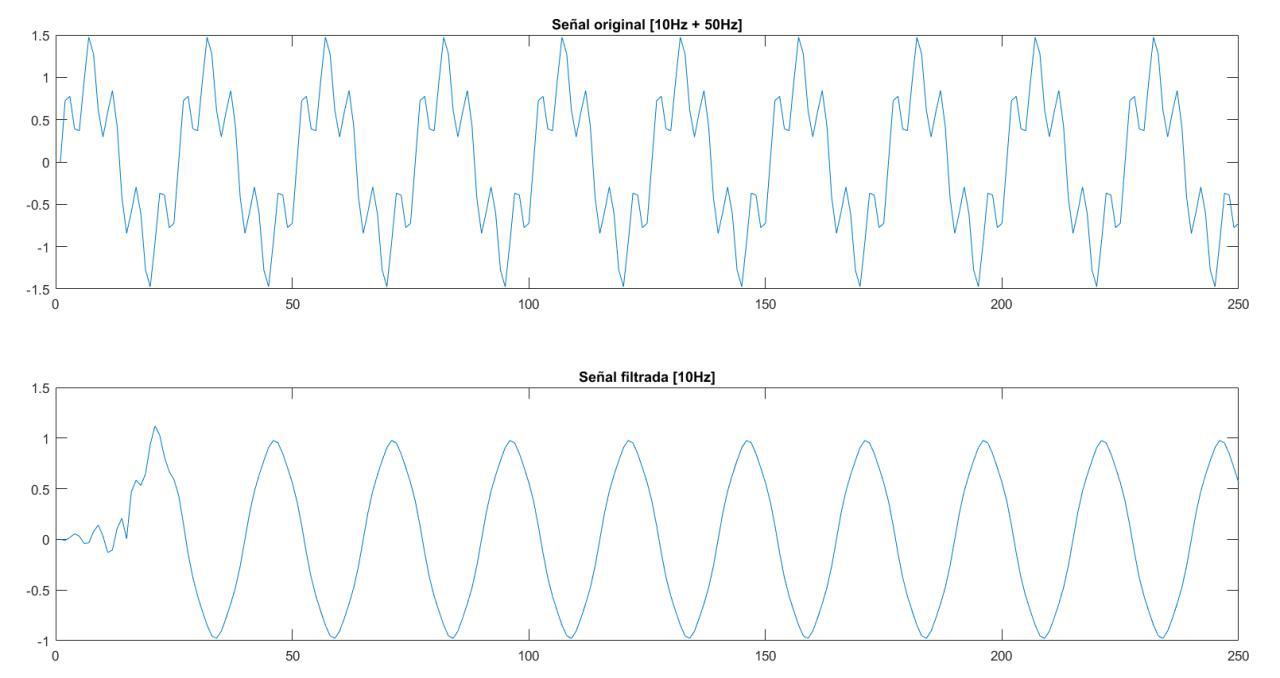
\includegraphics[width=16cm]{Notch_Matlab}
    \caption{Simulación del efecto del filtro Notch a 50Hz}
    \label{fig:Notch_Matlab}
\end{figure}

Como se puede observar, la componente de 50Hz ha sido eliminada casi por completo a costa de afectar ligeramente a la amplitud de la señal original. Tras comprobar que el resultado es satisfactorio se procedió a realizar una implementación del mismo filtro haciendo uso de CMSIS-DSP y el microcontrolador STM32F4.

Al no contarse con generadores de señales capaces de producir una señal de estas características se optó por generar una señal artificial con MatLab y almacenarla en la memoria del STM en la fase de programación. La figura \ref{fig:Filtro_en_STM} muestra la señal original (a) y la señal tras aplicarle el filtro (b).

\begin{figure}[H]
  \begin{subfigure}[b]{8cm}
   	\centering
    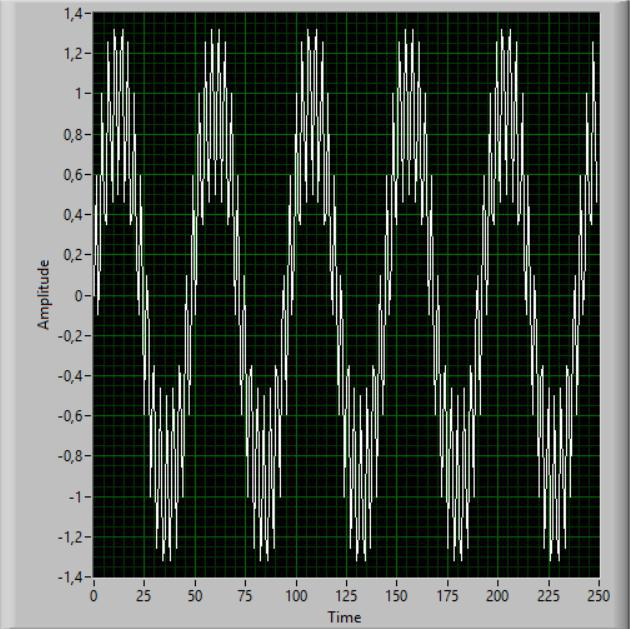
\includegraphics[width=8cm]{senal_original}
    \caption{Señal original con ruido de 50Hz}
    \label{fig:senal_original}
  \end{subfigure}
  \hfill
  \begin{subfigure}[b]{8cm}
  	\centering
    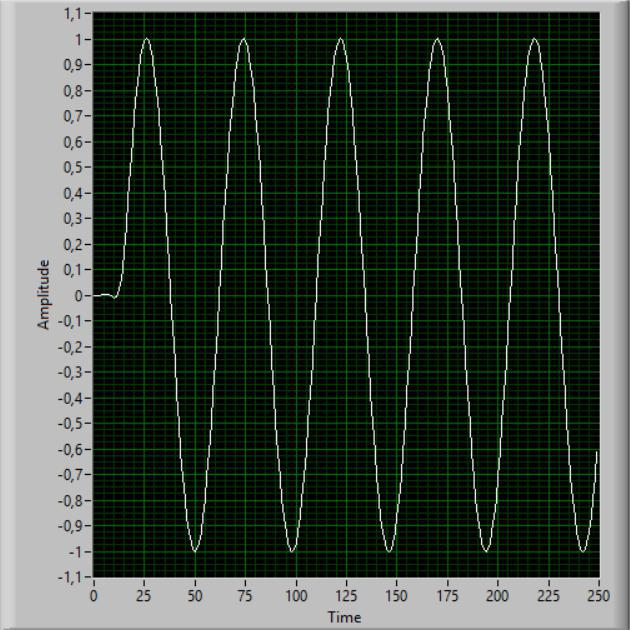
\includegraphics[width=8cm]{senal_filtrada}
    \caption{Señal filtrada}
    \label{fig:senal_original}
  \end{subfigure}
  \caption{Implementación real del efecto del filtro Notch a 50Hz}
  \label{fig:Filtro_en_STM}
\end{figure}

Tal y como se esperaba, la señal de 50Hz ha sido eliminada completamente, siendo los resultados obtenidos prácticamente idénticos a los simulados.

El diseño del filtro fuerza a que las componentes en frecuencia cercanas a 50Hz se vean más atenuadas que aquellas más alejadas. Las siguientes figuras muestran señales de 5Hz, 10Hz, 50Hz y 65Hz y como el cambio de frecuencia afecta a la amplitud de la señal.

\begin{figure} [H]
    \centering
    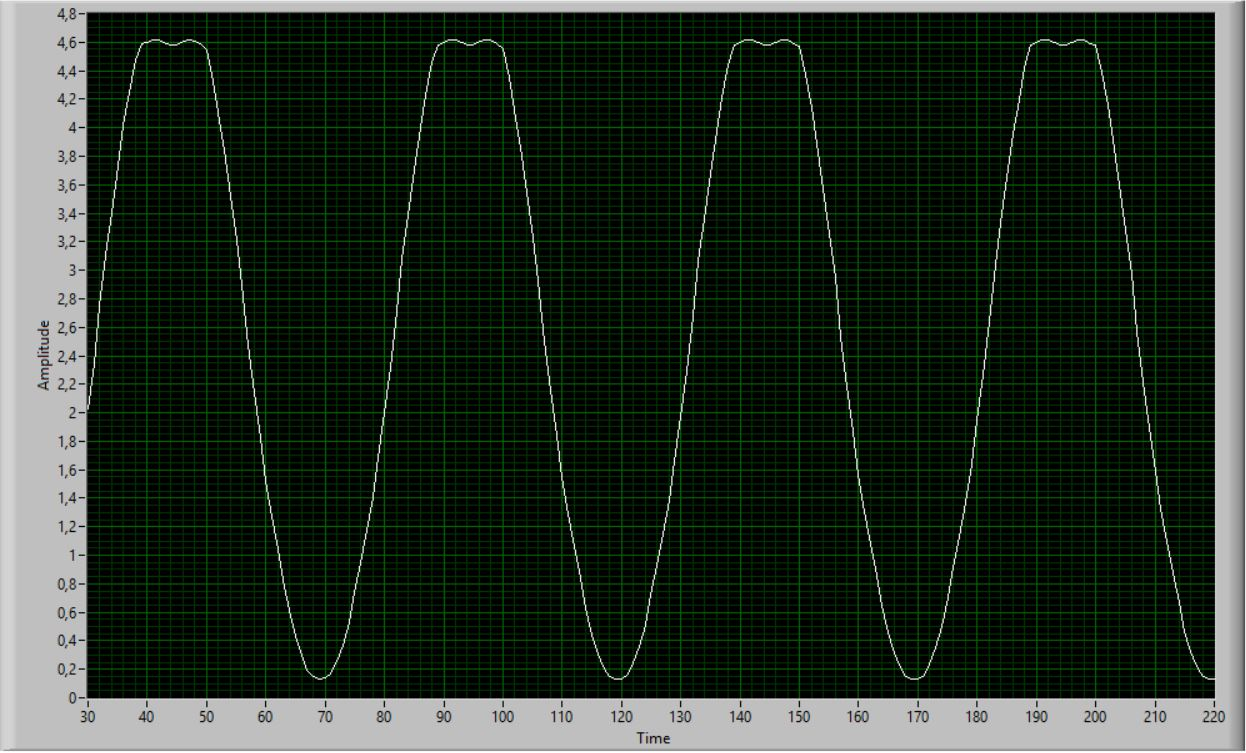
\includegraphics[width=15cm]{seno_5Hz}
    \caption{Señal de 5Hz filtrada}
    \label{fig:seno_5Hz}
\end{figure}

\begin{figure} [H]
    \centering
    \includegraphics[width=15cm]{seno_10Hz}
    \caption{Señal de 10Hz filtrada}
    \label{fig:seno_10Hz}
\end{figure}

\begin{figure} [H]
    \centering
    \includegraphics[width=15cm]{seno_50Hz}
    \caption{Señal de 50Hz filtrada}
    \label{fig:seno_50Hz}
\end{figure}

\begin{figure} [H]
    \centering
    \includegraphics[width=15cm]{seno_65Hz}
    \caption{Señal de 65Hz filtrada}
    \label{fig:seno_65Hz}
\end{figure}

El sistema está cumpliendo su función, pues ha atenuando claramente la señal de 50Hz mientras que las demás se mantienen con una amplitud similar a la original.

\clearpage

\section{Medida de un EEG real\label{Resultados_EEG}}

Las siguientes figuras representan un EEG medido usando la placa de adquisición tras el filtrado de la componente de 50Hz.

\begin{figure} [H]
    \centering
    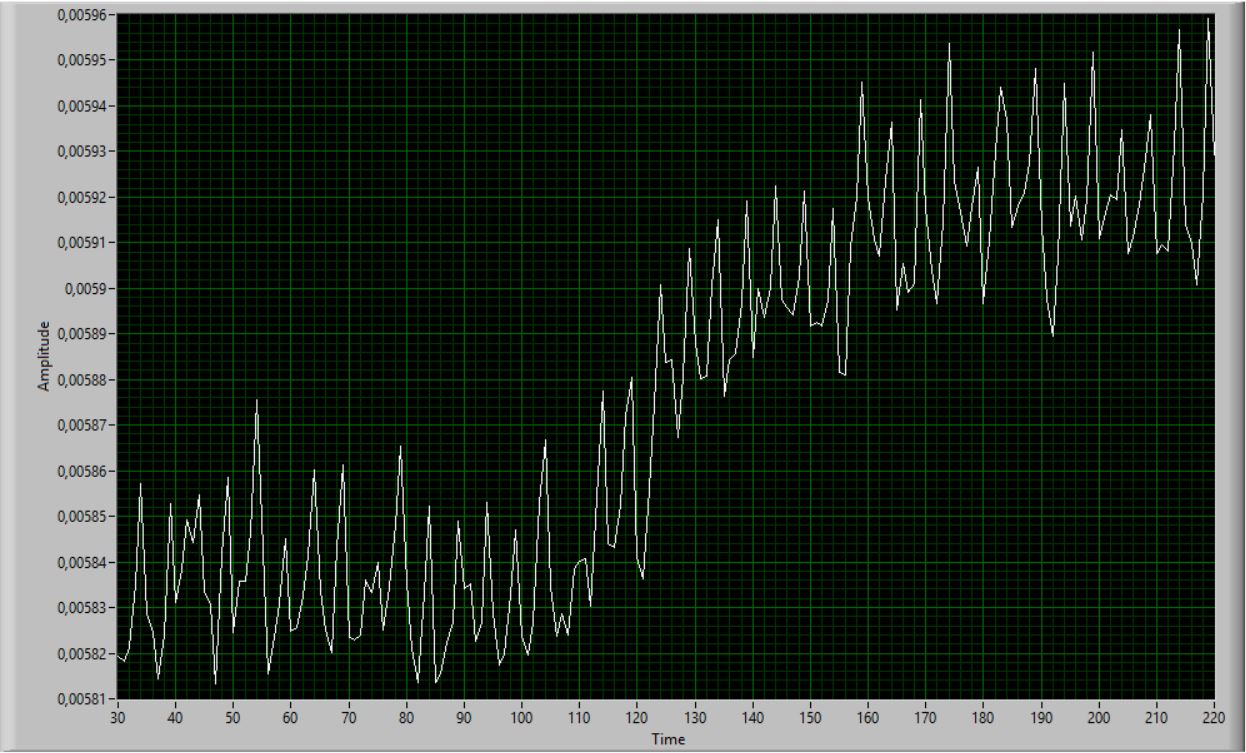
\includegraphics[width=15cm]{Medida_real_1}
    \caption{EEG abriendo los ojos}
    \label{fig:Medida_real_1}
\end{figure}

\begin{figure} [H]
    \centering
    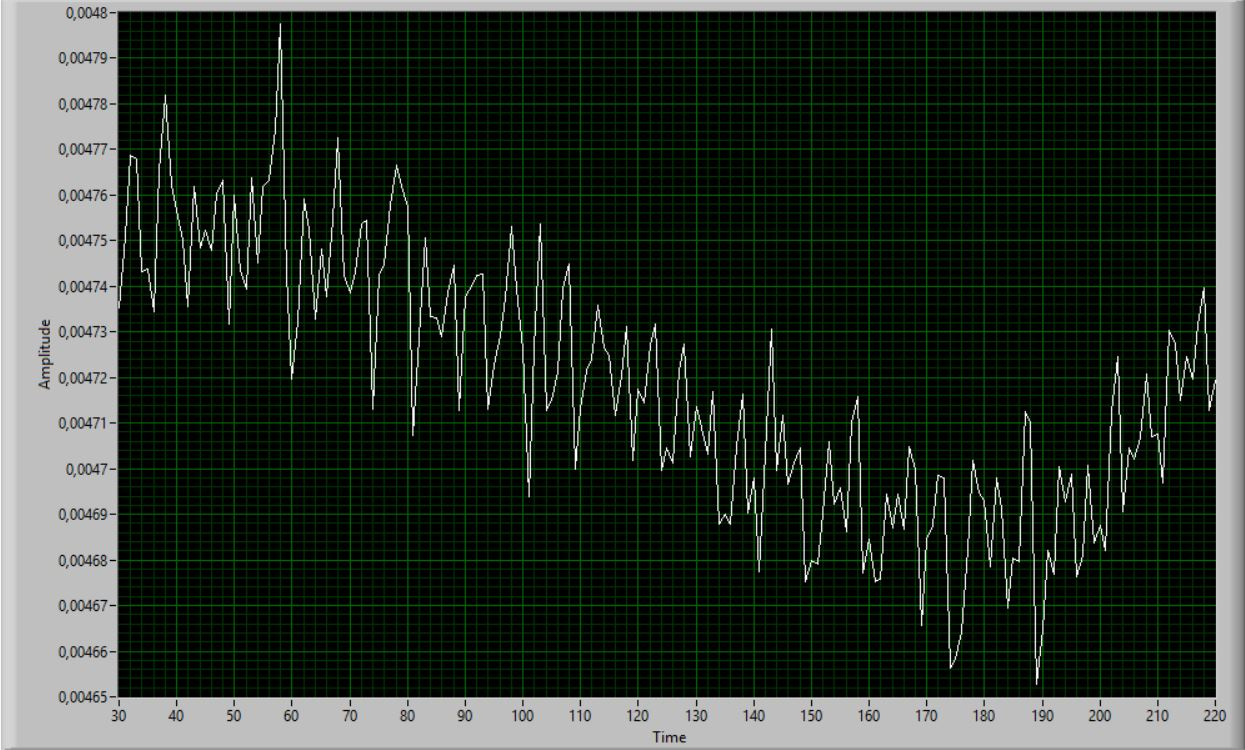
\includegraphics[width=15cm]{Medida_real_2}
    \caption{EEG con los ojos cerrados}
    \label{fig:Medida_real_2}
\end{figure}

A pesar del filtrado que se ha implementado aún se sigue observando una fuerte componente en frecuencias cercanas a los 50Hz. Esto se debe en gran parte a los sistemas de medida utilizados, ya que la presencia de cables tan largos, finos y con tan poco blindado los convierte en antenas perfectas para captar ruido de esa frecuencia. 

La figura \ref{fig:Sistema_medida} muestra el sistema de medida utilizado para adquirir estas señales.

\begin{figure} [h]
    \centering
    \includegraphics[width=10cm]{usuario_con_diadema}
    \caption{Sistema de medida utilizado para la adquisición del EEG}
    \label{fig:Sistema_medida}
\end{figure}

\section{Transmisión de datos por WiFi\label{Resultados_UDP}}

Por último se incluirán los resultados obtenidos mediante la transmisión de información por TCP y UDP a través de WiFi.

La librería WiFi del ESP contienen un gran número de funciones relacionadas con la transmisión de información tanto por UDP como por TCP.
Con el objetivo de transmitir los datos de la forma más fiable posible se optó por transmitirlos a través de TCP, pues este protocolo tiene sistemas que aseguran que el paquete llegará al destino.

Sin embargo utilizar este protocolo se tradujo en un tiempo de transmisión por cada 250 muestras superior a los 2 minutos haciendo inviable su uso.

En vista de la eficiencia de transmisión conseguida con TCP se utilizó UDP para la transmisión de la información al ordenador. Haciendo uso de este sistema la transmisión se completaba en apenas 1 segundo pero no todos los paquetes llegaban. Tras un poco de investigación se observó que cuanto mayor fuese el retardo introducido entre paquetes menos paquetes se perdían así que se afinó la transmisión hasta conseguir una tasa de transferencia lo suficientemente rápida con una pérdida de paquetes mínima.

\clearpage

En las siguientes imágenes se muestran tres casos en los que se transmitieron 100 paquetes que contenían variables de tipo float, el retardo utilizado entre paquetes y el porcentaje de paquetes perdidos.

\begin{figure}[h]
\centering
  \begin{subfigure}[b]{7cm}
   	\centering
    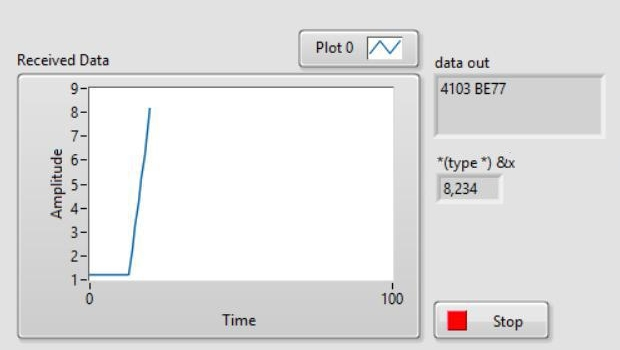
\includegraphics[width=7cm]{UDP_FAST_LOST}
    \caption{Sin retardo, 92\%}
    \label{fig:UDP_FAST_LOST}
  \end{subfigure}
  \begin{subfigure}[b]{7cm}
  	\centering
    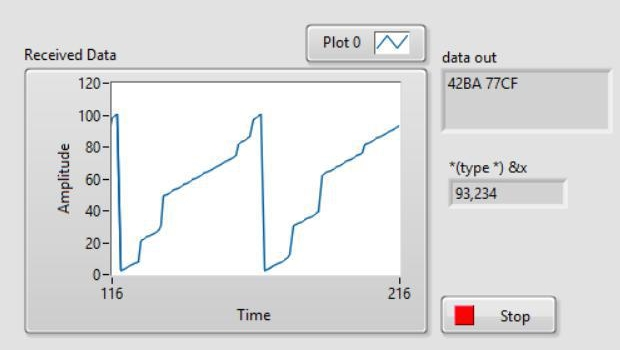
\includegraphics[width=7cm]{UDP_MEDIUM_MEDIUM}
    \caption{Retardo de 1ms, 10\%}
    \label{fig:UDP_MEDIUM_MEDIUM}
  \end{subfigure}
    \begin{subfigure}[b]{7cm}
  	\centering
    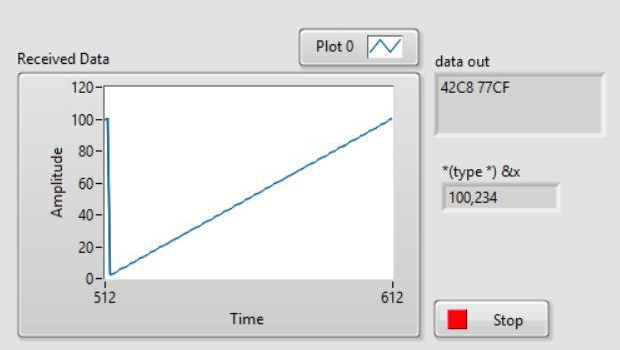
\includegraphics[width=7cm]{UDP_SLOW_LOW}
    \caption{Retardo de 5ms, sin pérdidas}
    \label{fig:UDP_SLOW_LOW}
  \end{subfigure}
  \caption{Comparativa entre los distintos retardos y el porcentaje de paquetes perdidos}
  \label{fig:LABEL}
\end{figure}

Con esta información se deduce que para que se reciban todas las muestras que se adquieren por segundo el tiempo de transmisión asciende a 1.25s (250 muestras * 0.005 segundos/muestra).

Este sistema sería ideal si entre transmisiones el sistema de adquisición capturase la siguiente muestra, pues permitiría montar un sistema de adquisición contínuo. Por desgracia esto no es compatible con el filtrado de la señal, al menos no directamente. Además la posibilidad de perder muestras es una característica no deseable.

Finalmente se realizó una segunda iteración sobre TCP, revisando en profundidad las librerías se detectó un error que provocaba un aumento en el tiempo de transmisión muy elevado (es importante recordar que dichas librerías no son oficiales y están en constante desarrollo por lo que la presencia de errores menores es algo habitual). Tras solventar dicho error el tiempo de transmisión de 250 muestras bajó a 1.28 segundos.

El resultado final es muy cercano al conseguido con UDP sin la posibilidad de perder muestras como ocurría con ese protocolo.